\documentclass{article}
\usepackage{amsmath, amsfonts, amsthm, amssymb}  

\usepackage{secdot}
\usepackage{epsfig}
\usepackage{cprotect}
\usepackage[T1]{fontenc}
\usepackage{epstopdf}
\usepackage{hyperref}
\usepackage{rotating}
\usepackage{graphicx}
\usepackage{caption}
\usepackage{subcaption}
\usepackage{multirow}
\usepackage{setspace}
\usepackage{array}
\usepackage{fancyhdr}
\usepackage{lastpage}
\usepackage[T1]{fontenc}

\usepackage{geometry}
\geometry{letterpaper, left=1in, right=1in, top=1in, bottom=1in}

\pagestyle{fancy}
\fancyhf{}
\rhead{\thepage/\pageref{LastPage}}
\lhead{OSU ECEN 2233 - Logic Design - Fall 2024}
\rfoot{\LaTeX}


% ----- Identifying Information -----------------------------------------------
\newcommand{\myassignment}{Lab 0: FPGA Basic Methodology}
\newcommand{\myduedate}{Assigned: Monday 8/19; Due \textbf{Monday 9/9} (midnight)}
\newcommand{\myinstructor}{Instructor: James E. Stine, Jr.}
% -----------------------------------------------------------------------------

\begin{document}
\begin{center}
  {\huge \myassignment} \\
  {\large \myduedate} \\
  \begin{flushright}
  \myinstructor \\
  \end{flushright}
\end{center}

\section{Introduction}

In this lab warmup, you will take a quick tour using the 
Verilog tools that we will use
in this class, and what it takes to run them by hand. You will then
construct a simple digital design in Verilog.
By the end of this warmup, you should be
familiar with MGC ModelSim for basic simulation and for viewing the
output of ModelSim. The laboratory is really meant to be an
easy-to-follow process of how to implement a design on a
Field-Programmable Gate Array (FPGA).

This laboratory albeit simple
is meant to familiarize yourself with the methodology in which we
design, validate and implement devices on our Field Programmable Gate
Array (FPGA) on the National Instruments DSDB board.  Therefore, it is
important to ask questions and learn as much as you can about the
process.  As we progress further throughout the semester, labs will
get progressively more difficult, so learn as much as you can with
this introductory laboratory.

\subsection{Simulation}

Simulation is key to making sure your hardware for any architecture or
digital system works.  It is often the difference between something
that works and something that is a pure speculation.  Therefore, it is
vital that for lab that you understand well how to simulate and get
results from ModelSim.

Although there are books and books out there on the subject, it is
best understood by someone who has been trained properly in the area.
It is also important you follow the right procedure which is summarized as
follows:
\begin{enumerate}
  \item Design the idea in Verilog to model as close as possible the
    implementation you wish to try.
    \item It is important you try to create the Hardware Descriptive
      Language (HDL) as close as possible to the final logic you wish
      to implement.  When you write HDL, it is not coding or software
      programming - it is modeling hardware.  The closer you make the
      HDL to the logic you wish to implement, the easier it will be
      for the synthesizer to complete the design.
    \item Write a testbench that will test your HDL you wish to test
      with known or golden vectors.
    \item Run the simulation with a script or DO (Tcl) file so
      that others can repeat the design if you wish.
    \item Although exhaustive simulation of your design is desirable,
      it is most often impossible;  therefore, test as many vectors as
      you can until the design works as properly.  If the design fails
      at any step, go back and test the lower-level hierarchy, if
      needed, to make sure it is working properly.
      \item After your design verifies through a testbench, implement
        your design on a FPGA.
\end{enumerate}

Mentor Graphics (MGC) ModelSim is a popular Hardware Descriptive
Language (HDL) compiler and
simulator that is widely used in the industry.  Although there are
similar tools form other vendors (e.g., Synopsys VCS or Cadence Design
Systems NCsim), the ideas are rather similar between Electronic Design
Automation (EDA) tools.  Regardless of the choice of simulator, the
use of testbenches and batch files to invoke simulation are the staple
of digital designers and architects.  

Testbenches are essential to HDL designs and they are not unique to
simulators.  They are part of the Verilog standard and are typically
written in a behavioral manner to make sure your simulation
essentially works.  Although many testbenches are utilized, using a
testbench that verifies what the \textbf{true} result should be is
essential.  Therefore, it is encouraged that you utilize a
self-checking style in your testbench.  Although testbenches are
usually written by the architecture, this part of the lab a sample
testbench is provided to you.  

The next part of the simulation environment is called a \verb+DO+ file
and is basically a batch file for ModelSim that allows the simulation
to run regardless of a users set up.  A sample \verb+DO+ file is given
to you, but you should modify to make sure it runs your finite state
machine design and its appropriate testbench.  To run ModelSim with a
\verb+DO+ file, type the following command at a command prompt.
\begin{verbatim}
vsim -do file.do
\end{verbatim}
It is encouraged to consult your TA or the Internet to learn how to get to
the terminal in Microsoft Windows, so you can run your DO file
correctly. 

\section{Full Adder Cell}

In the main part of this lab, you will construct a $1$-bit
full adder design using a Sum of Products (SOP) form.  This
circuit outputs a $1$-bit sum and a $1$-bit carry out for its input
$a$, $b$, and $c_{in}$.  The full adder is one of the more popular
pieces of digital logic that is utilized in most digital systems
today.  
This laboratory is really simple and meant to get you to go through
the process of understanding what is needed to implement the design on
a FPGA.

Often we start with a truth table that shows the output value for each
input combination. For an $n$-input function, a truth table has $2^n$
rows ($8$ in this case), one for each input combination. Each row lists
the output of the circuit for that input combination ($0$ or $1$ for a
one-bit output).  
The Boolean logic for the generation of an output indicating the sum
and carry out
of your $3$-bit (i.e., $a$, $b$, and $c_{in}$) input.  
To help you with the design and getting started, here is the following
Boolean logic that produces the correct answer.  However, it is
advisable to create a truth table of your inputs and outputs so you
can check whether your design works later in the laboratory.  
\begin{eqnarray*}
  sum & = & a \oplus b \oplus c_{in} \\
  c_{out} & = & a \cdot b + a \cdot c_{in} + b \cdot c_{in}
\end{eqnarray*}

\subsection{Requirements}

The HDL you write for this code should implement the Boolean logic for
your design given the equation above.
As explained in class, synthesis will typically optimize
your design to give you a different, realizable design and may or may
not look similar to the original HDL you designed.
Your module should contain $3$ inputs, ($a$, $b$, and $c_{in}$), each of
which hold $1$
bit each. It should have have one output port that indicates whether your
input number is the sum and carry out of your number.  Commercial
designers sometimes refer to the full adder as a $(3,2)$ counter
because it counts the number of inputs that are a $1$.  You should
verify this with your truth table.

\subsection{HDL Creation and Simulation}

Go ahead and write a Hardware Description (HDL)
module with the specification given above, and
build a testbench for your register file. In order to help you get
started, your repository should have an empty HDL file that is
missing some pieces.  However, it should have the ports to help you
figure out what is an input or output.  There is
an abundant amount of information in Chapter 4 in your
textbook~\cite{ddca-riscv} including some information on creating
the HDL for the full adder.

A testbench is another form of a HDL that is used to make sure your
design is designed correctly.  It basically tests all possible cases
against your design, typically called a $design under test$ or
\verb!dut!.
You should examine the sample
\verb!silly! testbench and use this to create a testbench for your
full adder.  More information is discussed on testbenches in your
textbook in Section~$4.9$ and discussed heavily in class.
Fortunately, you will use a simple testbench for this laboratory and
we will use subsequent labs to understand more complex testbenches.

Ensure that you test all
reasonable cases (e.g., $8$ possible values) before you implement the
design in a FPGA. Use the
waveform viewer in ModelSim in order
to examine the behavior of your design.  You should use modify
the testbench and \verb+DO+ file to help you verify your design
properly.

\subsection{Synthesis and Implementation}

As explained in class, when you synthesize a design it converts your
HDL from a known working piece of digital logic into one in which can
be implemented on the FPGA board.  We will use the Digital System
Development Board or DSDB board that inserts into the National
Instruments (NI) ELVIS-III
board.  This DSDB board contains an advanced FPGA with many
features that we will not fully utilize, however, it will still be able to
utilize all the features we require for our laboratories.

Another important note here is that before you begin the
implementation, your design should work without a hitch in
simulation.  Therefore, it is important to have your \textbf{working}
version of Verilog before you try to implement anything.  Do not waste
time implementing your design on the FPGA until it completely works in
simulation.  If for some
reason, your design does not work, it will be sure to not work in the FPGA.

For the synthesis and place \& route portions of the design flow, we
will use a tool called Vivado produced by Xilinx.  It should be
located on your desktop or through the application menu.  The goal at
the end of the day is to have the FPGA be assembled into a real, live
system. You start by writing Verilog and integrating IP and the result
is a bit file which gets loaded onto the FPGA and configures all of
its internal interconnects to implement your design. Starting with
correct code, this entire process can take anywhere from a few minutes
to hours depending on the complexity of the design. All “builds” are
broken into three main steps:

\subsubsection{Synthesis}

Generally, this is pretty quick (except for initial first-time). In
this step the System Verilog and other content (including block
diagram IP, interconnects, etc) are interpreted and built into a
synthesizable system that can be simulated (if desired). Synthesis is
where syntax issues in your SystemVerilog are caught as well as
blatant connection conflicts or things like combinatorial loops (cases
where a logic gate drives itself with no flip-flops/latches in
between). Synthesis does not look into timing restrictions or how a
particular line will get turned into an actual constructed device
using resources on the chip. That is usually determined in the next
step, Implementation.

\subsubsection{Implementation}

This is where the bulk of a “build” cycle will be spent. In this
step, the successfully-synthesized project (previous step) will be
laid out using the on-chip resources of the FPGA. It is an iterative
process which tries to optimize many variables in order to fit it on
the chip. Small designs can be implemented quickly, but larger designs
will take longer. The larger a design is relative to the resources on
a chip, the longer the implementation step will take since it has
less breathing room. Implementation will provide a resource-level
view of your entire design (down to the individual Lookup tables
(LUTs) in the design as well as show where everything is laid out on
the chip). Timing information will also be provided and timing
violations (e.g., violation of setup and hold requirements) will be
indicated here.

\subsubsection{Bitstream}

Usually, this is quick after the slog of the Implementation. Here the
implementation results from the previous step are converted into a
binary file that can be loaded into the FPGA and used to set up its
internal circuitry correctly.
In this lab, you will be using the
Digital System Development Board (DSDB) on an NI ELVIS-III
workstation. The DSDB contains a \verb!ZYNQ XC7Z020CLG484-1! FPGA.  In
Vivado, set the family to \verb!Zynq-7000!.

The quickest step by far is programming the device. This will take a
few seconds and pipes the
binary file of the previous step onto the FPGA as well as triggers a
few restart/configuration pins to make it automatically load. These
few seconds are the best seconds of your life. You've successfully
gotten a design through all the steps, but it has not yet let you down
by not working. Savor them. It doesn't get any better than this.

\section{What to design?}

As explained previously, you will be using the DSDB board.  The DSDB
board contains our Xilinx Zynq FPGA (Item~$18$ in Figure~\ref{dsdb1})
as well as other elements to help you
debug what is going on.  The diagram of the design is shown in
Figure~\ref{dsdb1}.
\begin{figure}
  \centering
  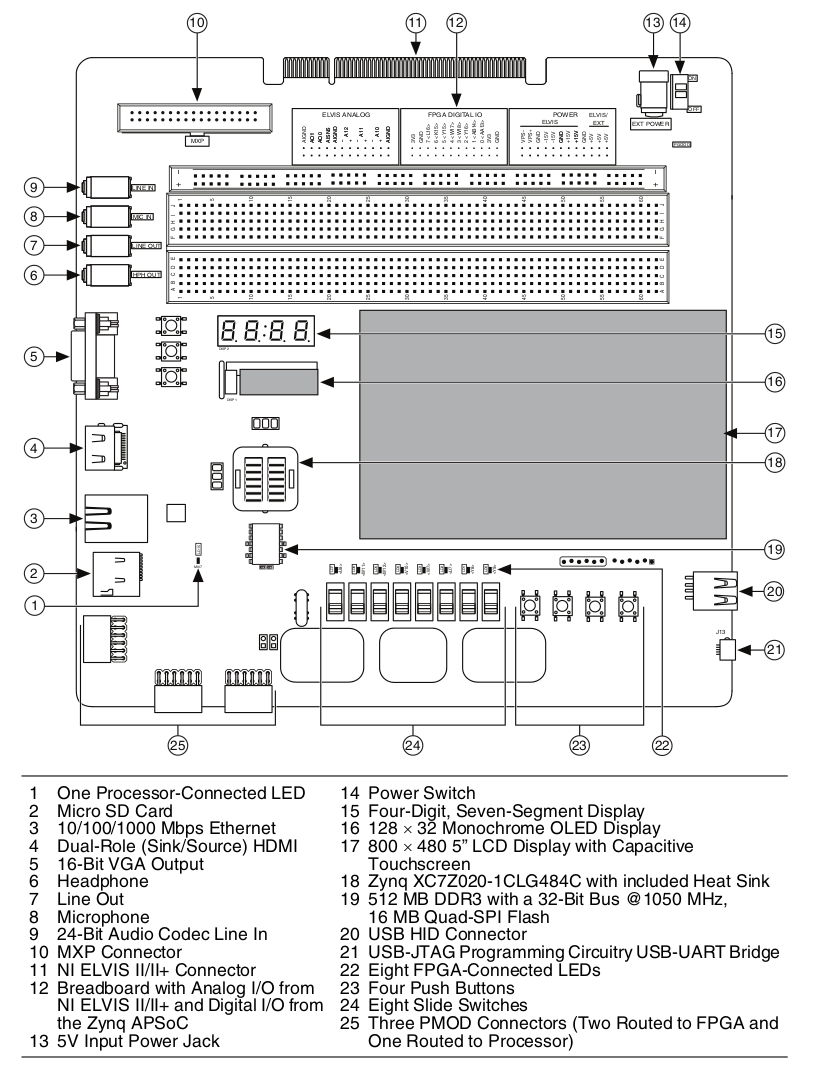
\includegraphics[scale=0.5]{dsdb1.png}
  \caption{The NI Digital System Development Board~\cite{dsdb1}}
  \label{dsdb1}
\end{figure}
For this laboratory, you will use the slide switches (Item~$24$ in
Figure~\ref{dsdb1}) to select the
inputs and the LEDs on board (Item~$22$ in Figure~\ref{dsdb1}) to see
if your design works properly.  Since there are only $3$ inputs, you
could test each possible combination of inputs to see if it matches
your truth table.

Hardware is difficult in that you really cannot see what is going on
within a design once it has been implemented.  Therefore, using your
brain and other elements to help figure out debugging problems is
important.  One of the most crucial elements of this, which is
something I hope you get from this laboratory, is the use of Light
Emitting Diodes or LEDs.  LEDs are silicon-based electronics that are
extremely invaluable for debugging designs.
For the remainder of the laboratories, you should remember to use LEDs
and switches throughout the semester as they will help you debug what
is happening when something it not working as expected.
And, LEDs may very well save
your professional life when implementing something as they can tell
what is happening at an output.  Today's electronics operate so fast
that its almost impossible to see what is happening.  Therefore, using
any visual cues to detect problems or issues is vital and engineers,
such as you and I and others everywhere,  
use this technique for that purpose.

The DSDB includes a four-digit seven segment display, eight slide
switches, four push buttons,
eight individual LEDs, and other unique I/O devices and breadboard
connections
connected to the Zynq FPGA.
%There is also one
%LED connected directly
%to the PS via MIO pin~$7$.
The push buttons and slide switches are
connected to the Zynq via series
resistors to prevent damage from inadvertent short circuits (a short
circuit could occur if a pin
assigned to a push button or slide switch was inadvertently defined as
an output). The push
buttons are “momentary” switches that normally generate a low output
when they are at rest, and
a high output only when they are pressed. The slide switches generate
constant high or low inputs depending on their position.

The eight high-efficiency LEDs are anode-connected to the Zynq via
$330~\Omega$ resistors, so they
will turn on when a logic high voltage is applied to their respective
I/O pin. A schematic is given of the DSDB board on Canvas for those
that are interested.  Additional LEDs
that are not user-accessible indicate power-on (\verb!PGOOD!), FPGA
programming status (\verb!DONE!), and USB and Ethernet port status.

You should use the following items for your ports in your top-level
module as shown in Table~\ref{ports.tbl}.  You do not have to use all
of the items, but they are there to use for inputs, outputs, or
debugging.  You should also test your design so it works for all $8$
combinations of inputs.
\begin{table}
  \centering
  \begin{tabular}{|c|c|c|c|c|} \hline
    Port & Type & Description \\ \hline \hline
    \verb!sw[3:0]! & Input & push buttons (\#23) \\ \hline
    \verb!btn[7:0]! & Input & SPDT slide switches (\#24)  \\ \hline
    \verb!led[7:0]! & Output & Light Emitting Diodes (LEDs) (\#22) \\ \hline
  \end{tabular}
  \caption{Ports Used for Lab~$0$}
  \label{ports.tbl}
\end{table}

\subsection{How to get started?}

To get you started there are a couple of downloads that will help you
get started.  All of these files are found within a zip file on Canvas
called \verb!lab0.zip!.
The first item is a complete SV file, testbench and DO
file you can use as a template for your test.  
Second, there is a zip
file of a demo program.  The demo program does not have anything in it
except a blank SV file that you should modify.  Feel free to modify
the file name or module name, if you wish, as well.

The included complete \verb!silly.sv! SV HDL file
is just a sample Verilog file that
implements a silly Boolean function (i.e., the same SV HDL file
found in Chapter~$4$ of your
textbook~\cite{ddca-riscv}).  A DO or Tcl file is a script
that simulates your design through ModelSim.
To simulate your \verb!silly.sv!,
go to a terminal and type:
\begin{verbatim}
vsim -do silly.do 
\end{verbatim}
You should use these
files, once you understand how to simulate something, to build the
required Verilog file for this laboratory (i.e., the full adder
circuit).

Once you design your SV of your full adder
and test it thoroughly, implement it on the
FPGA board.  It is important that your design work in simulation
\textbf{before} you even go to implementing on your FPGA board.
This should be fairly easy if you use the demo program
(i.e., zipped file) to insert your file into the design.
That is, once inside Vivado, open the unzipped file by navigating
through \verb!File->Project->Open! and opening the \verb!Demo.xpr!
project.  Once the project has opened, go to the \verb!top_demo.sv!
source by double-clicking the \verb!top_demo!
design.  It should look like Figure~\ref{demo} and 
you can now replace your ModelSim-tested HDL into the
\verb!top_demo! SV file. You can either copy your working HDL into the
\verb!top_demo! SV file or instantiate your full adder as discussed in
class.  Once
inserted, then synthesize and implement your design.  Synthesizing and
implementing your design on the FPGA normally takes several minutes
and so this is why we spend so much time designing our HDL before we
get to this step.
\begin{figure}
  \centering
  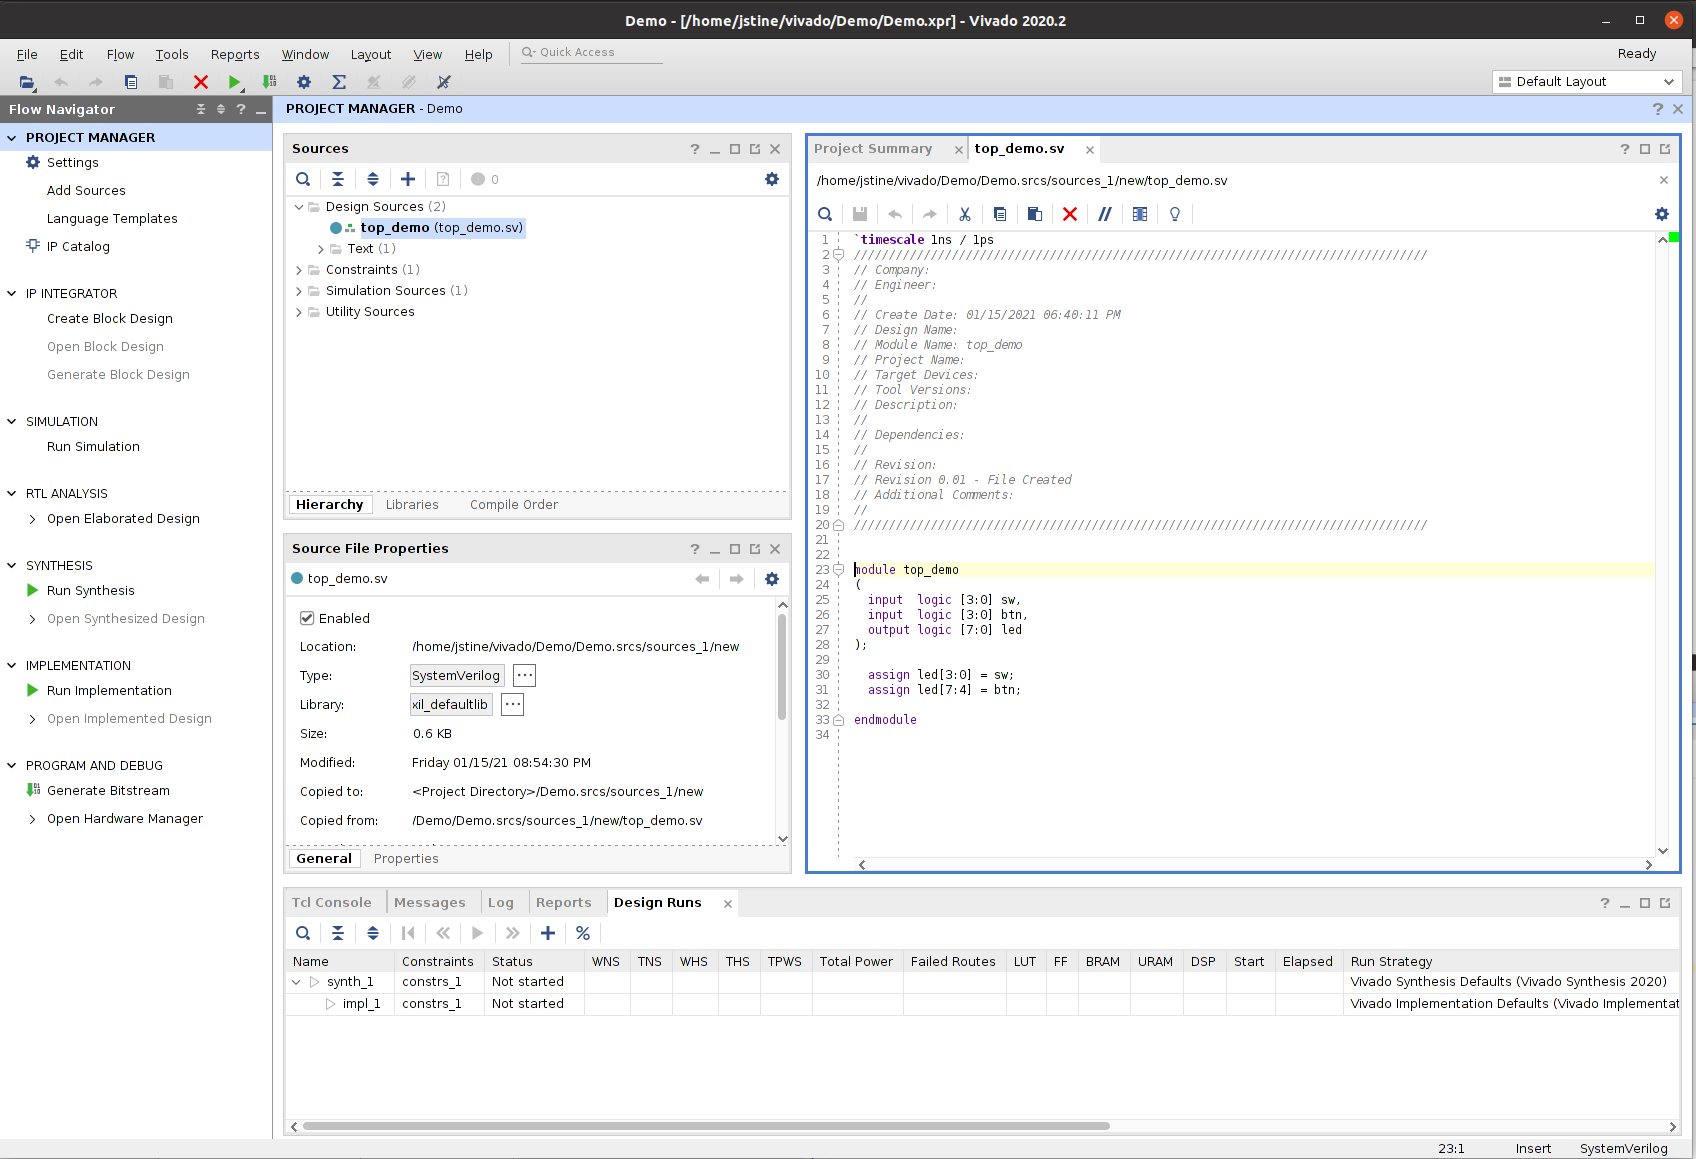
\includegraphics[scale=0.2]{top_demo.png}
  \cprotect\caption{The \verb!top_demo! opened project inside Xilinx Vivado}
  \label{demo}
\end{figure}

The Xilinx Vivado software is very complex and its going to take a
while to understand how to get more complicated designs through.  For
now, first make sure your SV completes the test correctly (i.e.,
through all $8$ combinations in ModelSim).  Then, when inside Vivado,
click the
following on the left-hand sidebar to start the process of
implementing onto the FPGA.
\begin{enumerate}
\item Run Synthesis
\item Run Implementation
\item Generate Bitstream
\end{enumerate}
This should
take a little bit of time, but once complete, the design should be
ready to download to the board.

To download to the board, click \verb!Open Hardware Manager! on the
left-hand sidebar and then you can either click \verb!Program Device!
on the left-hand sidebar or at the top of the screen.
Once implemented, the device should be running.
Then, use the LEDs and buttons to test
your design to see if it works as your simulation did.  You can also,
if needed, print out a schematic of your design by clicking the
\verb!Schematic! option under the \verb!RTL Anlaysis! section on the
left-hand sidebar.

As we learned in class, comnbinations is a selection of items from a
collection.  You only have two options per input, which amounts to
$2^3 = 8$ possible combinations of inputs.  Make a table of all $8$
possible input combinations and their respective output for the
implementation using the LEDs to help debug what is going on.  You
should keep a record of this testing to make sure things worked as
expected.  The output should match the testing you saw in your
ModelSim simulation.  That is, you should test the $8$ possible input
combinations in ModelSim \textbf{and} in the implementation on the
FPGA. Both versions of testing should match indicating your design
worked as indicated.

\subsection{FPGA Implementation}

You should also skim the document~\cite{7086413} and understand the
differences between what an Application-Specific Integrated Circuit
(ASIC) and a FPGA is.  This document is also in the repository,
so you should download and read it lightly, paying special
attention to Section II wihin the paper.
Both ASICs and FPGAs are extremely similar in
their structure, but can be different in terms of
their implementation.  However, they both use HDLs and using the
methodology discussed in class benefits both implementations.
Inside your lab report, you
should indicate why FPGAs are important and how they can be utilized
to implement digital gates efficiently.  Also, discuss what
advantages/disadvantages do FPGAs have?

\subsubsection{Power, Performance and Area (PPA)}

Digital systems typically employ outputs that indicate statistics of
how much space and time is consumed on a device.  These are typically
alotted into an analysis called Power, Performance and Area (PPA)
analysis.  You should document in your report how much PPA is utilized
for your final design.

During synthesis Vivado takes many of your HDL constructs and
translates them to their implementation.  As a designer, it is
important to keep your design as similar as possible to what the
digital logic represents.  However, there is a good chance that your
HDL usage may not look similar to the implemented design.  This is
because Xilinx Vivado
as well as many other synthesis programs utilize High-Level Synthesis
(HLS).  Right now, only commercial tools truly support HLS, but there
more synthesis programs in the future will support HLS.  Fortunately,
Xilinx Vivado truly supports HLS.

For future laboratories, we will explore the PPA of your design, but
for this lab you should only report your final area for your final design.
The area for the Xilinx FPGA is reported in 
``slices'' utilized.  You can find this information by ``Open
Implemented Design'' on the left side of the screen and then clicking
the ``Report Utilization'' tab, as seen in
Figure~\ref{utilization.fig}.    
This should produce output that
gives the total number of ``slices'' used for your design.
Interestingly, you can also look at the Schematic it produces by
clicking the Schematic option on the ``Open Implemented Design'' tab.
For these laboratories, you should just report the total ``Slices''
for your design.  This is a little harder to find, but its probaby
easy to see on the ``Design Runs'' tab at the bottom of the screen.
LUTs are the look-up tables discussed in~\cite{7086413}.
\begin{figure}
  \centering
  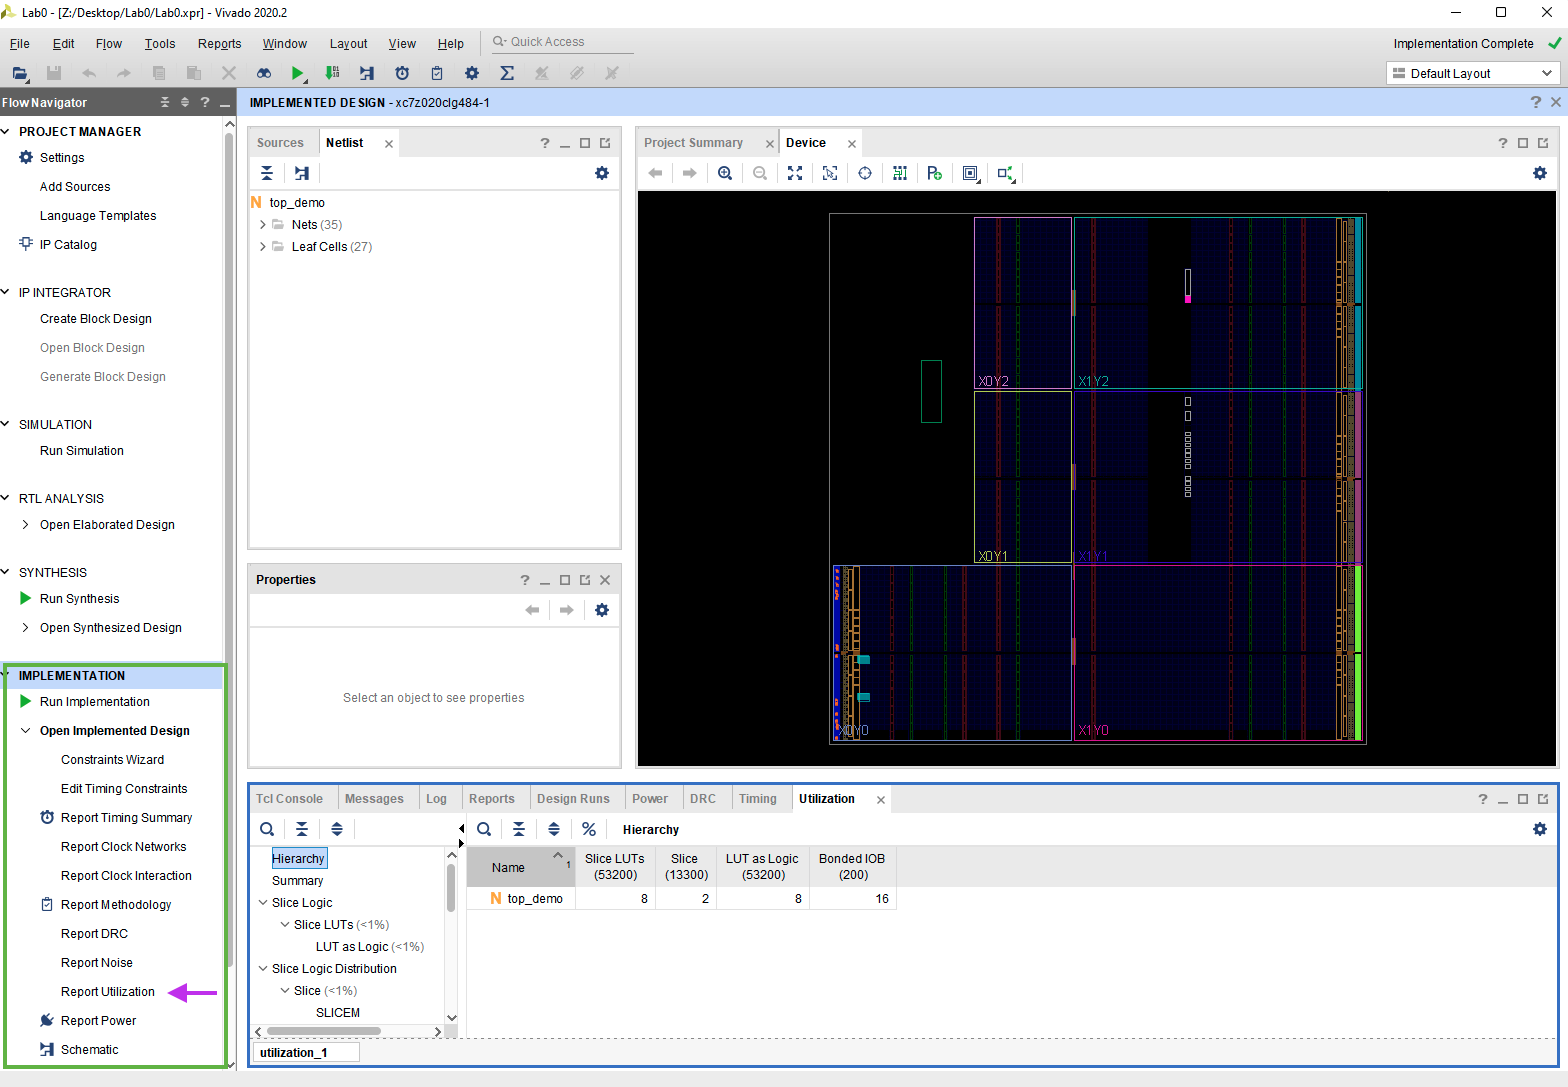
\includegraphics[scale=0.2]{Utilization.png}
  \caption{Implementation Window on Xilinx's Vivado}
  \label{utilization.fig}
\end{figure}


\section{Handin}

You should electronically hand in your HDL (\textbf{all} files that you want
us to see) into Canvas.
You should also take a printout of your waveform 
from your ModelSim simulation.  This lab should be done \textbf{individually}
and will differ from the other laboratories that will invovle your
team members. 
Please contact
the James Stine (james.stine@okstate.edu) 
for more help.  Your
code should be
readable and well-documented. In addition, please turn in additional
test cases or any other added item that you used. 
Please also remember to document everything in your Lab Report using
the information found in the Grading Rubric.

\bibliographystyle{IEEEtran}
\bibliography{lab0}

\end{document}
